\documentclass[uplatex]{jsarticle}
\usepackage{amsmath}
\usepackage[dvipdfmx]{graphicx}

\setcounter{tocdepth}{3}
\usepackage{float}
\usepackage{moreverb}
\usepackage{lscape}
%\pagestyle{empty}
%\usepackage{wrapfig}
\usepackage{url}
%\usepackage{EasyLayout}

\usepackage{ascmac}
%\usepackage{fancybx}

%\pagestyle{myheadings}



\begin{document}

\begin{flushright}
    \number\year 年\number\month 月\number\day 日
\end{flushright}

\begin{center}
    {\LARGE アイディアソンポスターセッション報告書}
\end{center}

\begin{flushright}
    グループ番号:01\\
    学生番号:25G1065\\
    氏名:塩澤匠生
\end{flushright}


\section{はじめに}
まず,社会的背景として自転車の単独事故は年5497件発生していて,その割合は年々増加している
というものがある\cite{jikokensuu}.
単独事故の割合は,年々増加しているというものがある.そして,
単独事故の原因の内7割が転倒事故であるというものがある\cite{tandokuWariai}.



ここで,車の単独事故の原因の内訳と比較してみると車の単独事故の内転倒(横転)事故は1\%
であることから,自転車は乗り物の性質上転倒事故が発生するという問題があると考えることができる.



\section{解決策としての提案手法}
自転車の性質上,転倒事故が発生しやすいという問題に対して我々は自転車姿勢制御モジュールというものを
提案する.自転車姿勢制御モジュールの概念図を以下図\ref{fig:moduleGainenn}に示す

\begin{figure}[H]
    \centering
    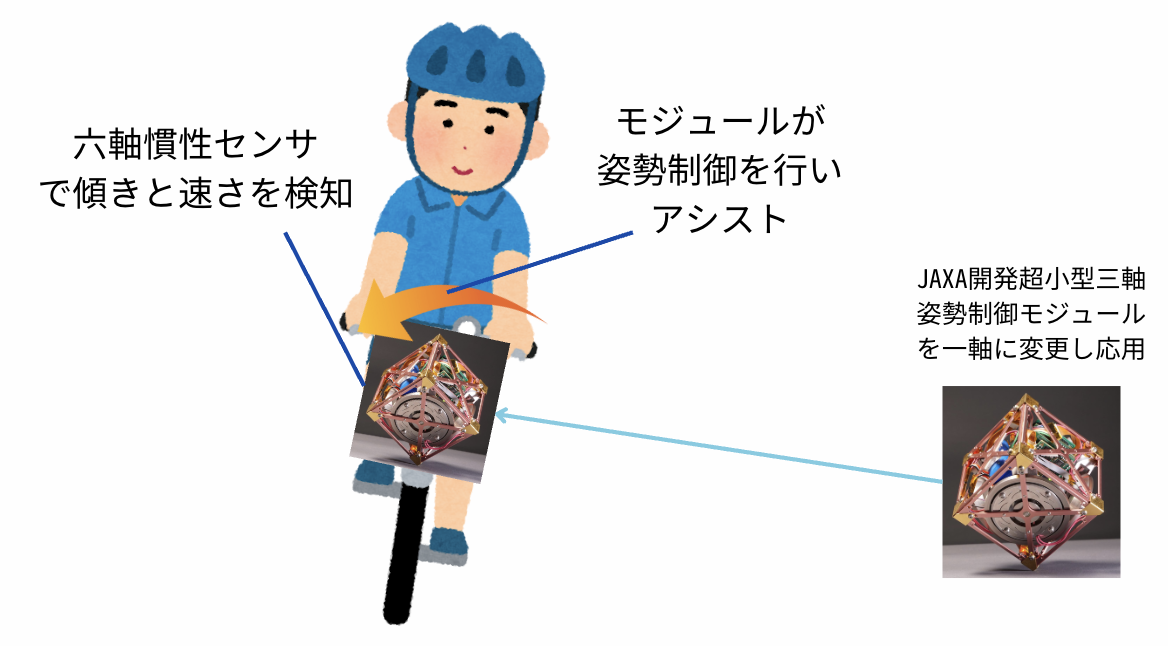
\includegraphics[width=0.8\textwidth]{fig/moduleGainenn.png}
    \caption{自転車姿勢制御モジュールの概念図}
    \label{fig:moduleGainenn}
\end{figure}

まず,先行研究として,JAXAが開発した超小型三軸姿勢制御モジュールというものがある.
このモジュールは人工衛星の小型化を図るために作られたものでサイズは$10×10×10 {cm}^3$である.



\begin{thebibliography}{9}

\bibitem{jikokensuu} NEONAVI, 【自転車事故の実態】を知って安全に利用しよう~令和5年「交通事故統計」から, 
2025年6月11日閲覧,\url{https://neonavi.info/11203/}

\bibitem{tandokuWariai} 東京海上日動, 便利な自転車は運転次第で危険な乗り物になる, 
2025年6月11日閲覧,\url{https://www.tokiomarine-nichido.co.jp/world/guide/drive/202105.html}\end{thebibliography}

\end{document}



























